\section{OrderView}

Im Order-View werden alle vom Nutzer getätigten Bestellungen angezeigt und können damit
jederzeit abgerufen werden.

\subsection{Render-Widget für Bestellungen}

Eine Bestellung wird, wie ein Menü, mithilfe eines individualisierten Card-Widgets
dargestellt.
Anstatt der bekannten Informationen des Menüs werden hier die wichtigen Daten der entsprechenden
Bestellung angezeigt\\
Dazu gehören:

\begin{itemize}
    \item das Datum der Bestellung
    \item die bestellten Waren
    \item der scanbare QR-Code der Bestellung
    \item der zu zahlende Betrag vor und nach Abzug des möglichen Rabattes
\end{itemize}

Jener QR-Code wird an der Kassa des Anbieters vom \nameref{adminclient} eingescanned, um einerseits
die bestellte Waren zu überprüfen und andererseits jene Bestellung abzuschließen und den Code
ungültig zu machen.

\begin{figure}[H]
    \centering
    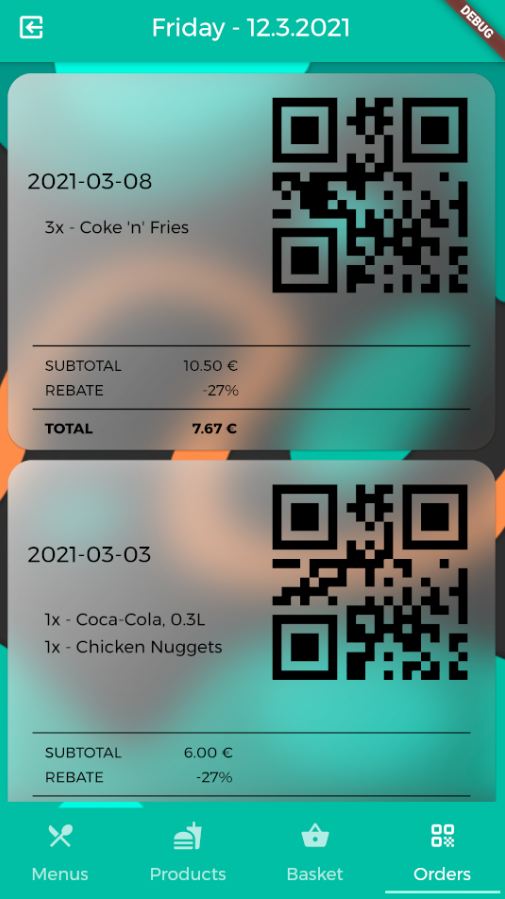
\includegraphics[width=0.40\textwidth]{images/Client/views/orderview/orderview.png}
    \caption{Order-View mit Card-Widgets für jede Bestellung}
\end{figure}

Damit das Scannen des QR-Codes an der Kassa vor Ort verbessert wird, kann der Code einer Bestellung
durch Antippen vergrößert werden. Hierfür wird ein \lstinline{ModalBottomSheet} mit weißem Hintergrund
geöffnet, auf dem das QR-Image in vergrößerter Form abgebildet und damit leichter einscanbar ist.

Da ein \lstinline{QrImage}-Widget allerdings kein definiertes \lstinline{onTap}-Property hat, muss
das onTap-Verhalten des QR-Codes mithilfe eines \lstinline{GestureDetectors} implementiert werden.

\begin{code}[H]
    \centering
    \includegraphics[width=1\textwidth]{images/Client/views/orderview/gesturedetector.png}
    \vspace{-20pt}
    \caption{Implementation der onTap-Funktionalität des QR-Codes}
    \label{gesturedetector}
\end{code}

\newpage

Nun kann durch kurzes Antippen der QR-Codes für den Scan vergrößert werden und sieht wie folgt
in der App aus:

\begin{figure}[H]
    \centering
    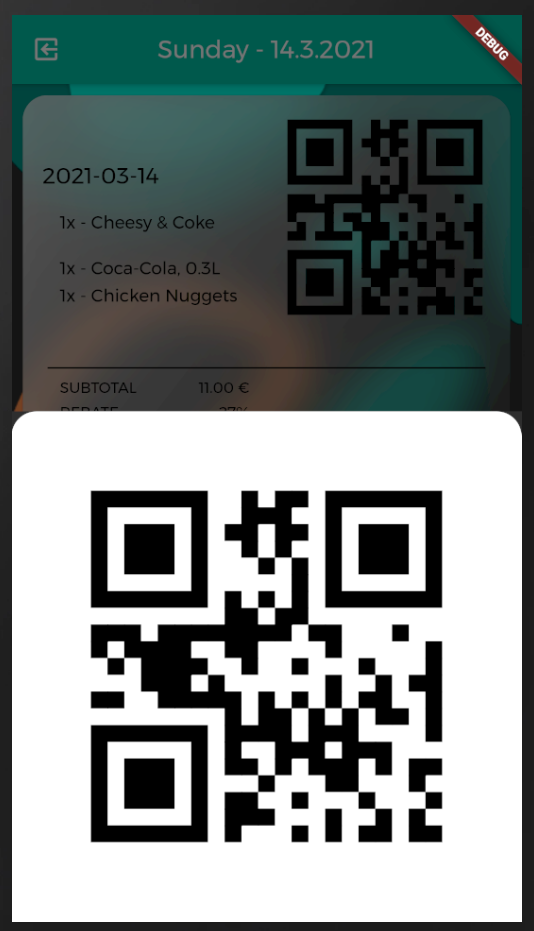
\includegraphics[width=0.40\textwidth]{images/Client/views/orderview/qrcode.png}
    \caption{Per Modal-Bottom-Sheet vergößerter QR-Code zum Erleichtern des Scans}
\end{figure}

\newpage

\subsection{Darstellen der Bestellungen im Order-View}

Dem Prinzip des \nameref{basketview}s folgend, werden auch im Order-View alle Bestellungen des Nutzers
in Form von Order-Panels generiert und mittels ListView.builder-Widget angezeigt.

Hat der Nutzer hingegen noch keine Bestellungen getägigt wird, auch hier das Sokka-Logo mit entsprechender
Meldung angezeigt.

\begin{figure}[H]
    \centering
    \hfill
    \subfigure[Order-View mit diversen vom Nutzer getätigten Bestellungen]{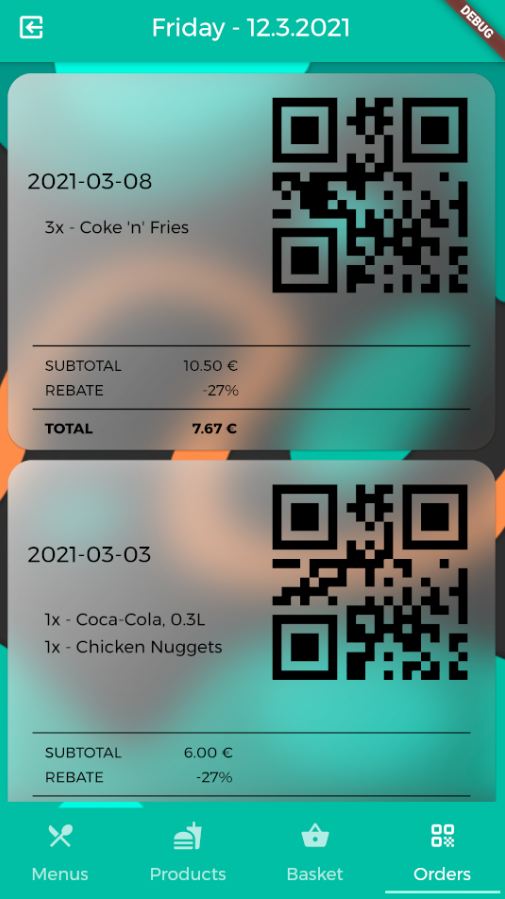
\includegraphics[width=0.4\textwidth]{images/Client/views/orderview/orderview.png}}
    \hfill
    \subfigure[Leeres Order-View]{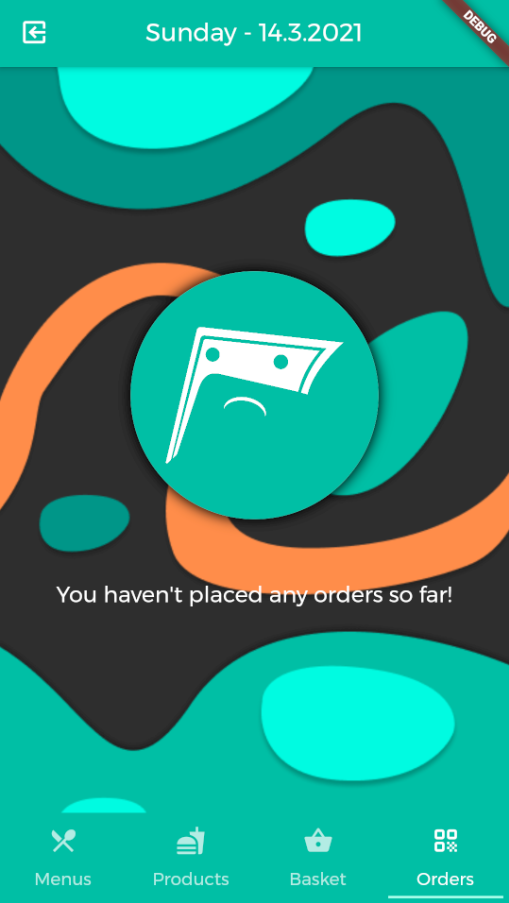
\includegraphics[width=0.4\textwidth]{images/Client/views/orderview/emptyOrders.png}}
    \hfill
    \caption{Leeres als auch befülltes Order-View}
\end{figure}